\documentclass[aspectratio=169, hideothersubsections]{beamer}
%\documentclass{beamer}
%\documentclass[aspectratio=1610]{beamer}
\usepackage{listings}
\usepackage{graphicx}
\usepackage{tikz}
\usetheme{Berkeley}
\usefonttheme{structuresmallcapsserif}
\usecolortheme{owl}
%\usepackage{xcolor}
%\usepackage{darkmode}
%\enabledarkmode
%\usecolortheme{albatross}
%\usecolortheme{spruce}
\usepackage{minted}
\usepackage{comment}
\usepackage{animate}  


\setbeamertemplate{page number in head/foot}[totalframenumber]
\setbeamertemplate{navigation symbols}{\footnotesize\usebeamertemplate{page number in head/foot}}
\setbeamercolor{title}{fg = OwlRed}
\setbeamercolor{author}{fg = OwlBlue}
%\setbeamercolor{frametitle}{fg=white}
%\setbeamercolor{background canvas}{bg=black}
%\setbeamercolor{normal text}{fg=white}

%--------------------------------------
%REPLACE IMAGE.JPG WITH LOGO OF ORGANISATION
\logo{\begin{tikzpicture}
\node[inner sep=0pt] at (0,0) {
\includegraphics[height=1cm]{SODS Logo.png}};
\end{tikzpicture}}
%--------------------------------------

\title{BSDS-210 : Business Intelligence and Data Analysis}
\subtitle{Course Instructor - Ms. Neema Jha}
\author[Gauri Sharan]{Gauri Sharan - BSc Data Science, Semester 4}
\date{June 11, 2024}

\begin{document}
\frame{\titlepage}

\begin{frame}{Table of contents}
    \tableofcontents[hideallsubsections]
\end{frame}

\section{Introduction to Tableau}
\begin{frame}{Introduction to Tableau}
  \begin{itemize}
    \item Tableau is a powerful data visualization tool.
    \item It helps in simplifying raw data into an understandable format.
    \item Data analysis is very fast with Tableau and the visualizations created are in the form of dashboards and worksheets.
  \end{itemize}
  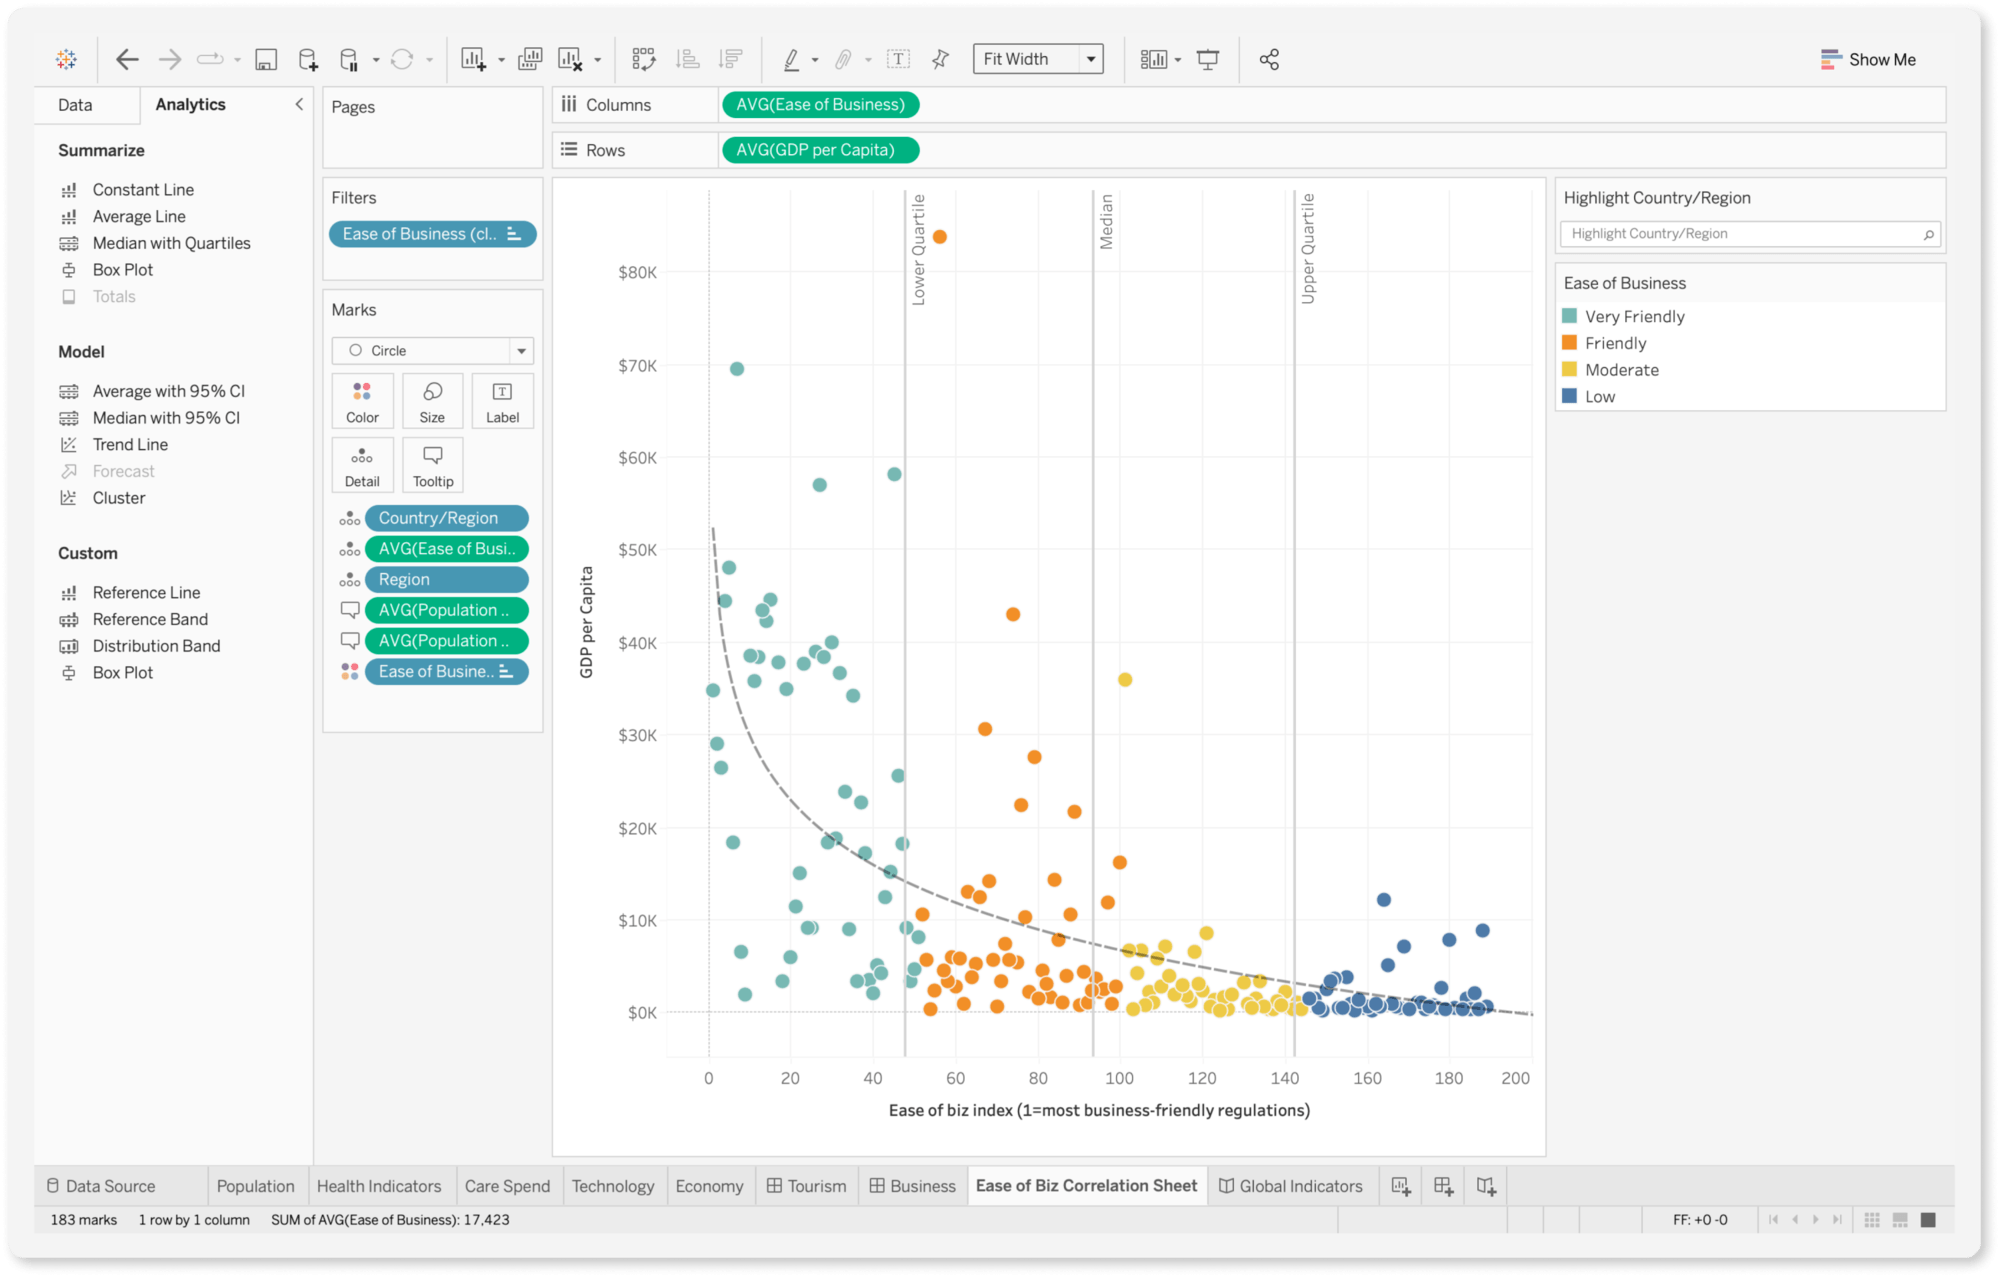
\includegraphics[width=\textwidth]{tab1.png}
\end{frame}

\subsection{Features of Tableau}
\begin{frame}{Features of Tableau}
In Tableau we can perform operations such as Data Blending, Real-time analysis, Collaboration of data etc.
\begin{figure}
  \centering
  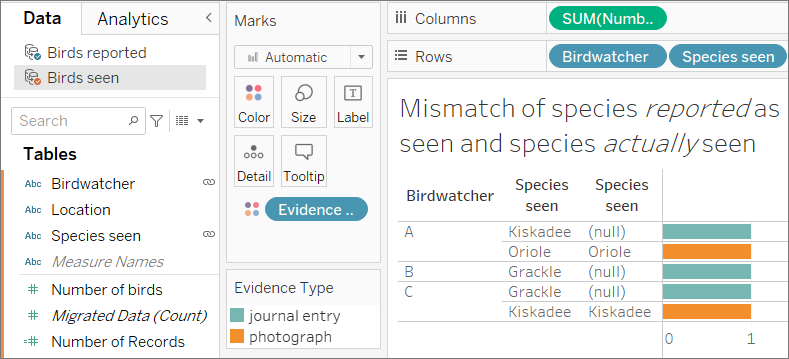
\includegraphics[width=0.6\textwidth]{tab2.png}
  \label{fig:example}
\end{figure}
\end{frame}

\subsection{Connecting to Data}
\begin{frame}{Connecting to Data}
  \begin{itemize}
    \item Tableau can connect to various data sources such as Excel, SQL Server, Google Sheets, and many more.
    \item The connection process involves connecting to data, preparing data, and analyzing data.
  \end{itemize}
 \begin{figure}
  \centering
  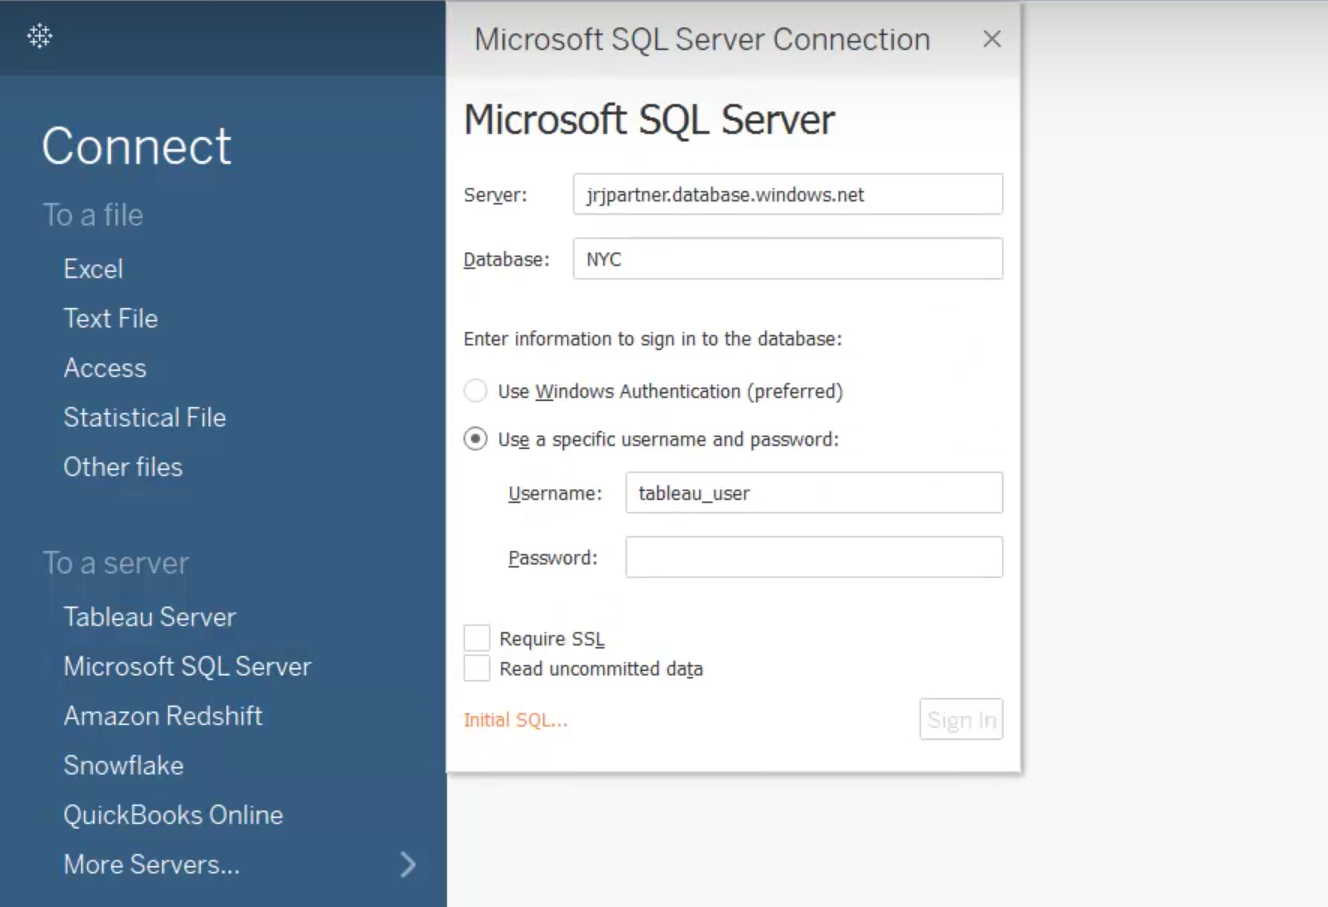
\includegraphics[width=0.5\textwidth]{tab3.png}
  \label{fig:example}
\end{figure}
\end{frame}

\subsection{Creating Visualizations}
\begin{frame}{Creating Visualizations}
  \begin{itemize}
    \item Visualizations in Tableau are created using various charts like bar charts, line charts, and pie charts.
    \item These charts help in analyzing data trends and patterns.
  \end{itemize}
 \begin{figure}
  \centering
  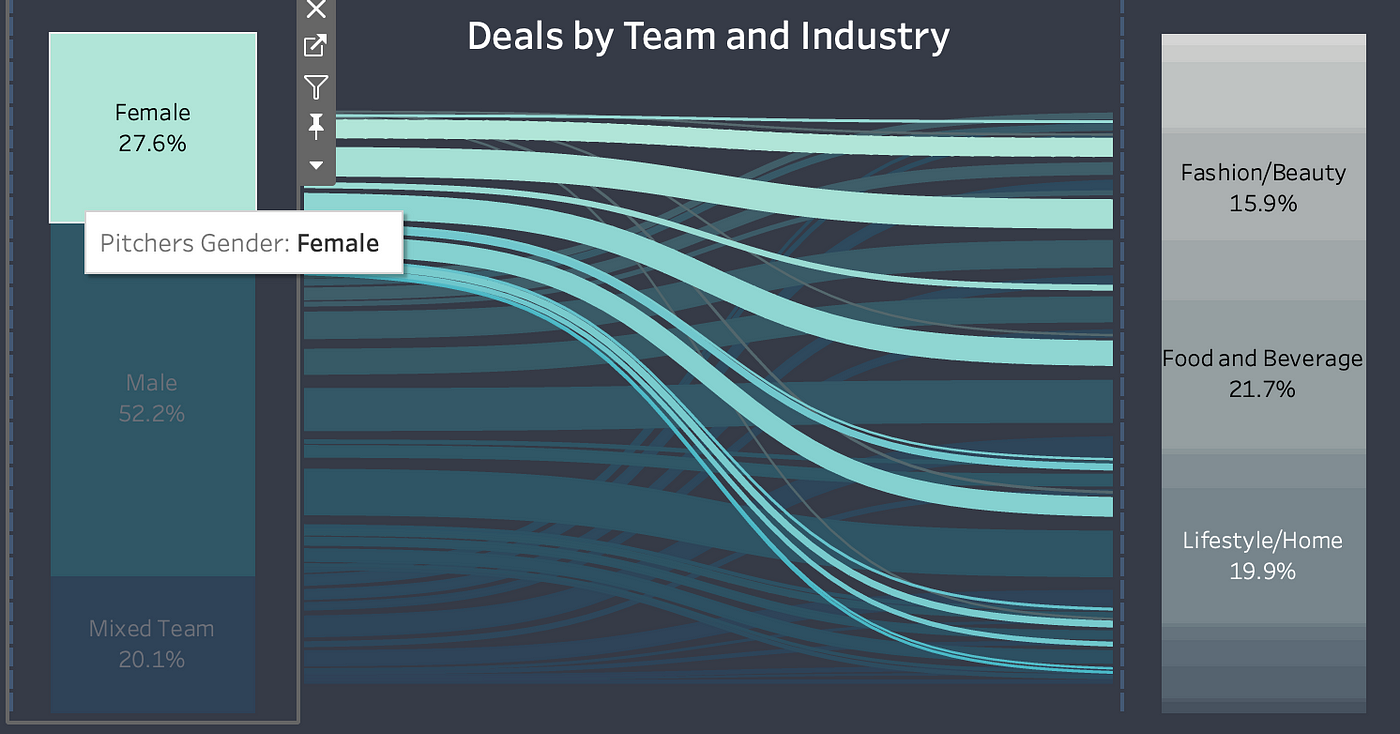
\includegraphics[width=0.5\textwidth]{tab4.png}
  \label{fig:example}
\end{figure}
\end{frame}

\section{Introduction to Power BI}
\begin{frame}{Introduction to Power BI}
  \begin{itemize}
    \item Power BI is a suite of business analytics tools.
    \item It connects to different data sources to analyze data and share insights.
  \end{itemize}
  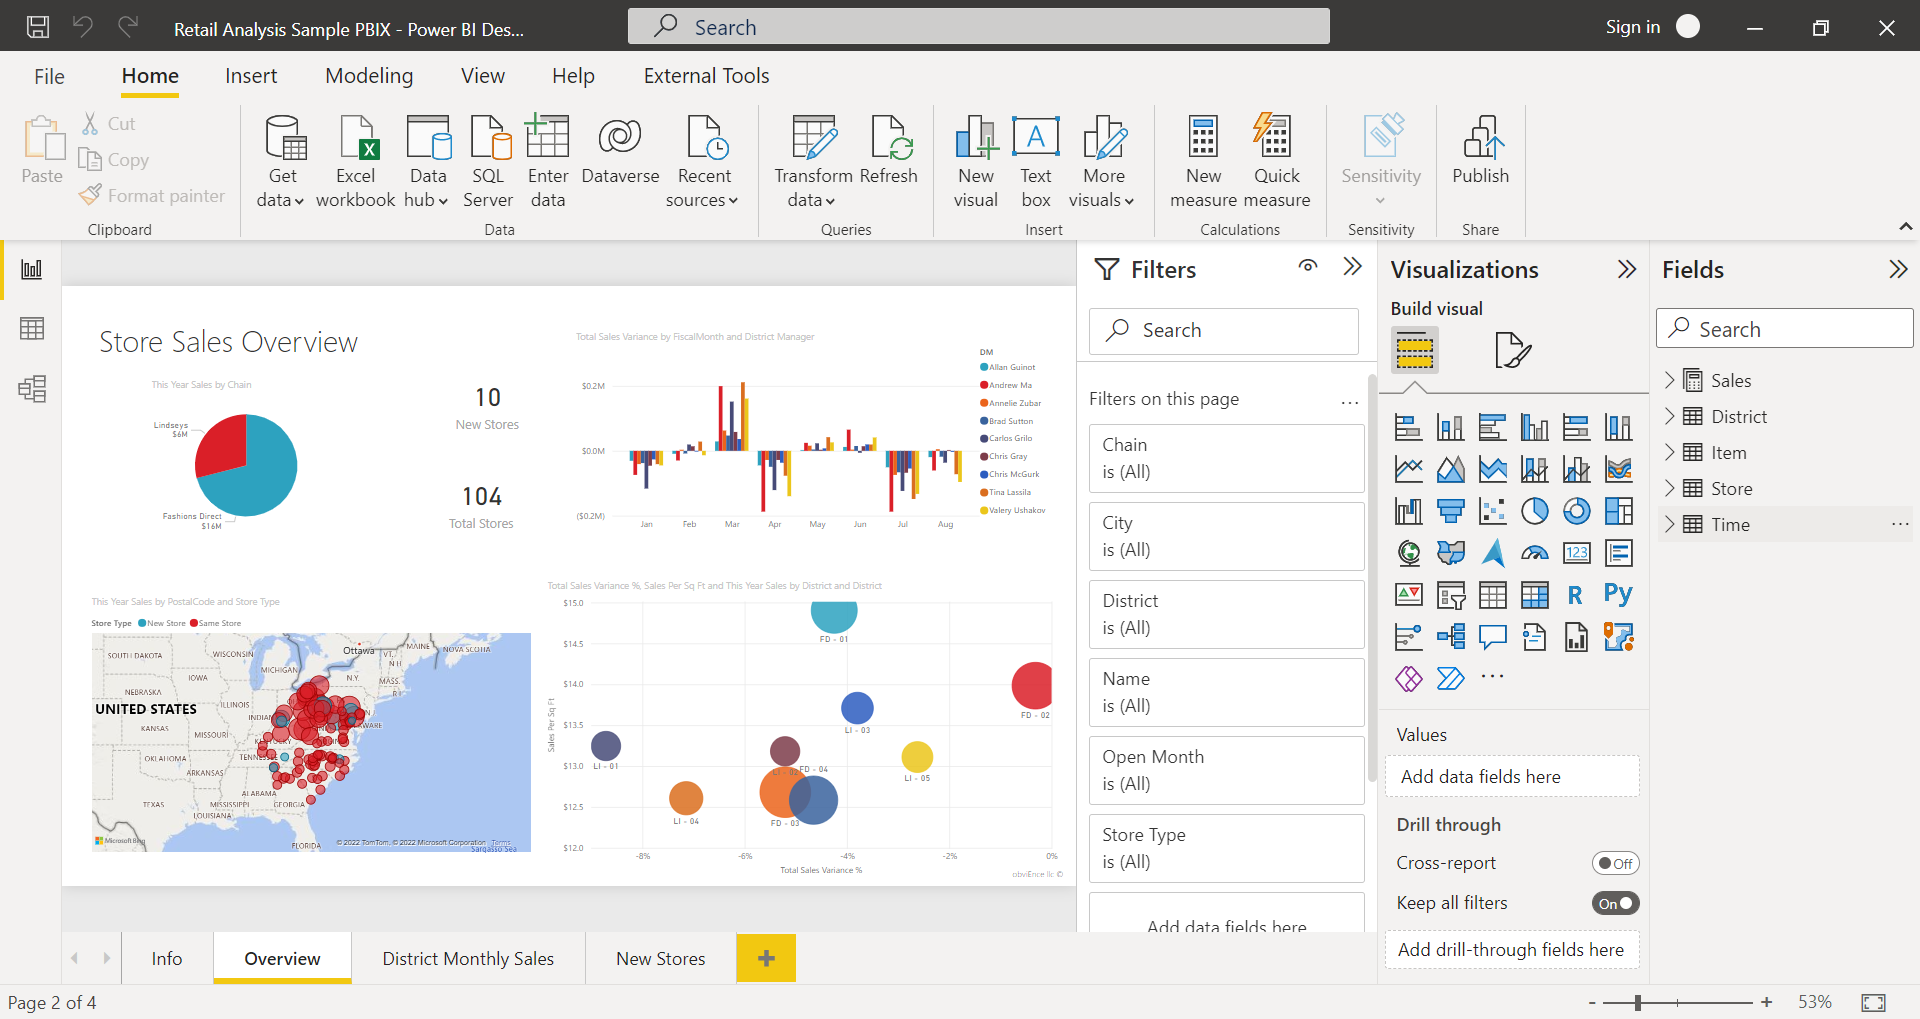
\includegraphics[width=\textwidth]{pb1.png}
\end{frame}

\begin{frame}{Parts of Power BI}
  \begin{itemize}
    \item Power BI Desktop
    \item Power BI Service
    \item Power BI Mobile
  \end{itemize}
 \begin{figure}
  \centering
  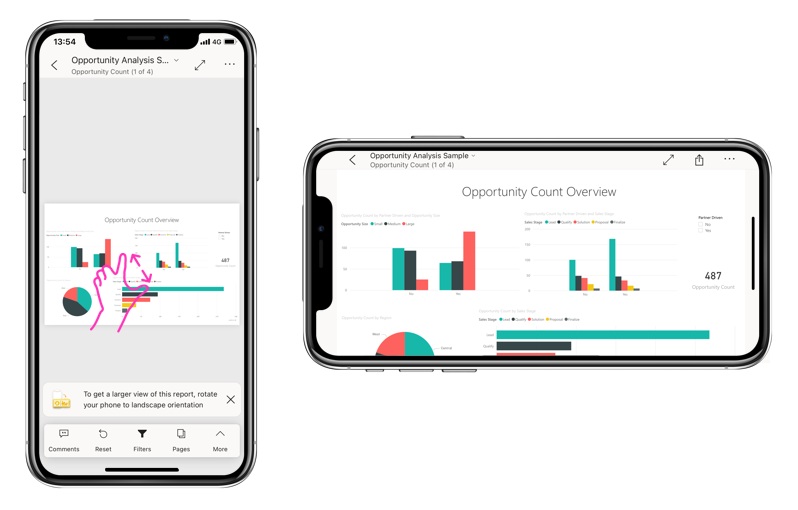
\includegraphics[width=0.5\textwidth]{pb2.png}
  \label{fig:example}
\end{figure}
\end{frame}

\begin{frame}{Power BI Desktop Interface}
  \begin{itemize}
    \item Ribbon: Displays common tasks associated with reports and visualizations.
    \item Pages: Allows selecting or adding a report page.
    \item Visualizations: Change visualizations, customize colors or axes, apply filters, and more.
    \item Fields: Drag and drop query elements and filters onto the Report view.
    \item Views Pane: Reports View, Data View, Relationship or Model view.
  \end{itemize}
\end{frame}

\subsection{Querying Data from CSV}
\begin{frame}{Querying Data from CSV}
  \begin{itemize}
    \item Import and clean data from various sources.
    \item Use the Query Editor to connect to one or many data sources, shape and transform the data.
  \end{itemize}
 \begin{figure}
  \centering
  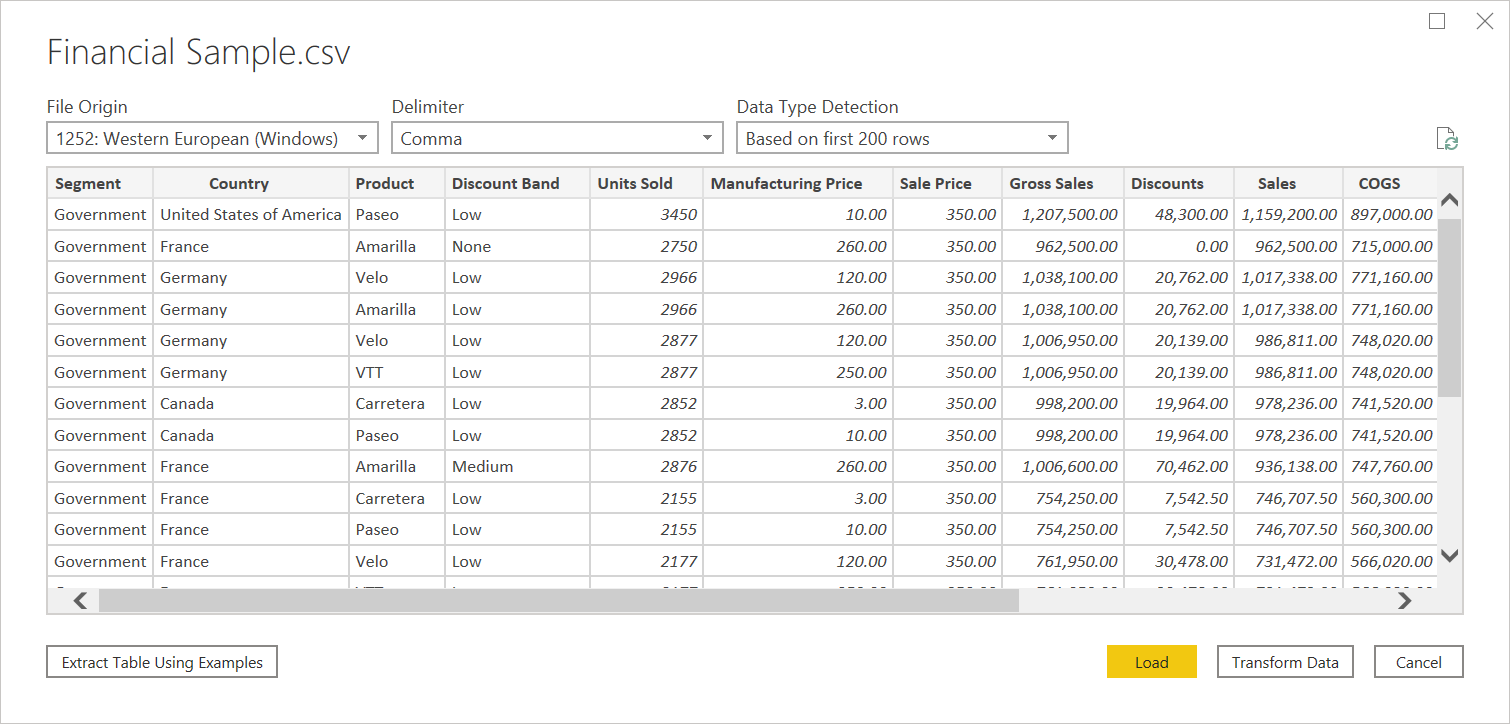
\includegraphics[width=0.6\textwidth]{pb3.png}
  \label{fig:example}
\end{figure}
\end{frame}

\subsection{Creating Reports \& Visualizations in Power BI}
\begin{frame}{Creating Reports \& Visualizations}
  \begin{itemize}
    \item Create visualizations such as bar charts, line charts, pie charts, and more.
    \item Use DAX for creating calculated measures.
  \end{itemize}
\begin{figure}
  \centering
  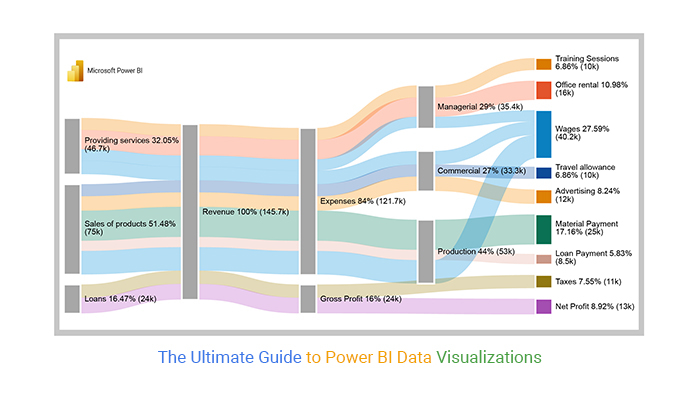
\includegraphics[width=0.6\textwidth]{pb4.jpg}
  \label{fig:example}
\end{figure}
\end{frame}

\section{References}
\begin{frame}{References}
  \begin{thebibliography}{10}
    \beamertemplatebookbibitems
    \bibitem{tableauref} Tableau Software. \textit{Official website}. \url{https://www.tableau.com}
    \beamertemplatebookbibitems
    \bibitem{powerbiref} Microsoft Corporation. \textit{Official website}. \url{https://powerbi.microsoft.com}
  \end{thebibliography}
\end{frame}

\section{Thank You}
\begin{frame}{Thank You}
Hope you liked this presentation. \newline \newline
\alert{Gauri Sharan} \newline
Student, School of Data Science \newline
AAFT Noida (Shobhit University) \newline
BSc Data Science 2022-25 \newline
Semester 4, 2024 \newline
\begin{itemize}
    \item LinkedIn: \href{https://www.linkedin.com/in/gauri-sharan}{\bf linkedin.com/in/gauri-sharan} 
    \item GitHub: \href{https://github.com/gaurisharan}{\bf github.com/gaurisharan}
    \item Mail: \href{mailto:gaurisharan123@gmail.com}{\bf gaurisharan123@gmail.com}
\end{itemize}
\end{frame}

\end{document}
